% Class Notes Template
\documentclass[12pt]{article}
\usepackage[margin=1in]{geometry} 
\usepackage[utf8]{inputenc}

% Packages
\usepackage[french, english]{babel}
\usepackage{amsmath, amsthm, amssymb ,amsfonts, graphics, tikz, float, enumerate}
\usepackage{listings}
\usepackage{color} %red, green, blue, yellow, cyan, magenta, black, white
\definecolor{mygreen}{RGB}{28,172,0} % color values Red, Green, Blue
\definecolor{mylilas}{RGB}{170,55,241}

\lstset{language=Matlab,%
	%basicstyle=\color{red},
	breaklines=true,%
	morekeywords={matlab2tikz},
	keywordstyle=\color{blue},%
	morekeywords=[2]{1}, keywordstyle=[2]{\color{black}},
	identifierstyle=\color{black},%
	stringstyle=\color{mylilas},
	commentstyle=\color{mygreen},%
	showstringspaces=false,%without this there will be a symbol in the places where there is a space
	numbers=left,%
	numberstyle={\tiny \color{black}},% size of the numbers
	numbersep=9pt, % this defines how far the numbers are from the text
	emph=[1]{for,end,break},emphstyle=[1]\color{blue}, %some words to emphasise
	%emph=[2]{word1,word2}, emphstyle=[2]{style},    
}

% Title
\title{ECON 6130 - Problem Set \# 4}
\date{\today}
\author{Julien Manuel Neves}

% Use these for theorems, lemmas, proofs, etc.
\theoremstyle{definition}
\newtheorem{example}{Example}[section]
\newtheorem{theorem}{Theorem}
\newtheorem{lemma}[theorem]{Lemma}
\newtheorem{proposition}[theorem]{Proposition}
\newtheorem{claim}[theorem]{Claim}
\newtheorem{axiom}[theorem]{Axiom}
\newtheorem{corollary}[theorem]{Corollary}
\newtheorem{remark}[theorem]{Remark}
\newtheorem{definition}[theorem]{Definition}
\setcounter{MaxMatrixCols}{20}

% Usefuls Macros
\newcommand\N{\mathbb{N}}
\newcommand\E{\mathbb{E}}
\newcommand\R{\mathbb{R}}
\newcommand\F{\mathcal{F}}
\newcommand\Z{\mathbb{Z}}
\newcommand\st{\text{ such that }}
\newcommand\seq[1]{\{ #1 \}}
\newcommand{\inv}{^{-1}}


\newcommand{\norm}[1]{\|#1 \|}
\newcommand{\inp}[2]{\langle #1, #2 \rangle}

\newcommand{\pa}[1]{\left(#1\right)}
\newcommand{\bra}[1]{\left[#1\right]}
\newcommand{\cbra}[1]{\left\{#1\right\}}

\newcommand{\pfrac}[2]{\pa{\frac{#1}{#2}}}
\newcommand{\bfrac}[2]{\bra{\frac{#1}{#2}}}

\newcommand{\mat}[1]{\begin{matrix}#1\end{matrix}}
\newcommand{\pmat}[1]{\pa{\mat{#1}}}
\newcommand{\bmat}[1]{\bra{\mat{#1}}}


\begin{document}

\maketitle

\section*{Part (1)}

For this problem set, we use the Adaptive Random-Walk Chain Metropolis-Hastings algorithm as defined in the notes with the following proposal density
\begin{align*}
	q(\Theta^*\mid \Theta^{(s-1)}) = N(\Theta^{(s-1)}, \Sigma_{s-1})
\end{align*}
where $\Sigma_{s-1}= 0.003 \cdot \Sigma_{\Theta s-1}$.

The prior distributions chosen for $\Theta$ are
\begin{align*}
	\sigma & \sim N(2,0.1)\\
	\beta & \sim B(.99,0.05)\\
	\phi & \sim N(4,0.1)\\
	\phi_{\pi} & \sim N(1.5,0.1)\\
	\phi_{y} & \sim N(0.125,0.1)\\
	\theta & \sim B(0.75,0.1)\\
	\alpha & \sim B\left( \frac{1}{3},0.1\right) 
\end{align*}
and improper distributions for the rest of $\Theta$.

These prior distributions usually come from micro data and stylized facts. Technically, we could use uninformative distributions for every parameters, but since we have more information about certain specific parameters it is better to incorporate this into our MCMC algorithm.

Note that the chosen prior distributions specific parameter values comes from the class notes.

N.B. I believe Prof. Nimark's code for the prior distributions is incorrect. There is a mismatch between the distributions and $\Theta$. This could explain the disparity between my results and the ones shown in class.


\section*{Part (2)}
With our choice of parameters for the Adaptive Random-Walk Chain Metropolis-Hastings algorithm, the acceptance rate is equal to roughly 20\%. This is roughly the sweet spot between too small steps/high acceptance rate and too big steps/low acceptance rate.

The raw MCMC for $\Theta$ is plotted in Fig. \ref{fig:raw}.

\begin{figure}[H]
	\centering
	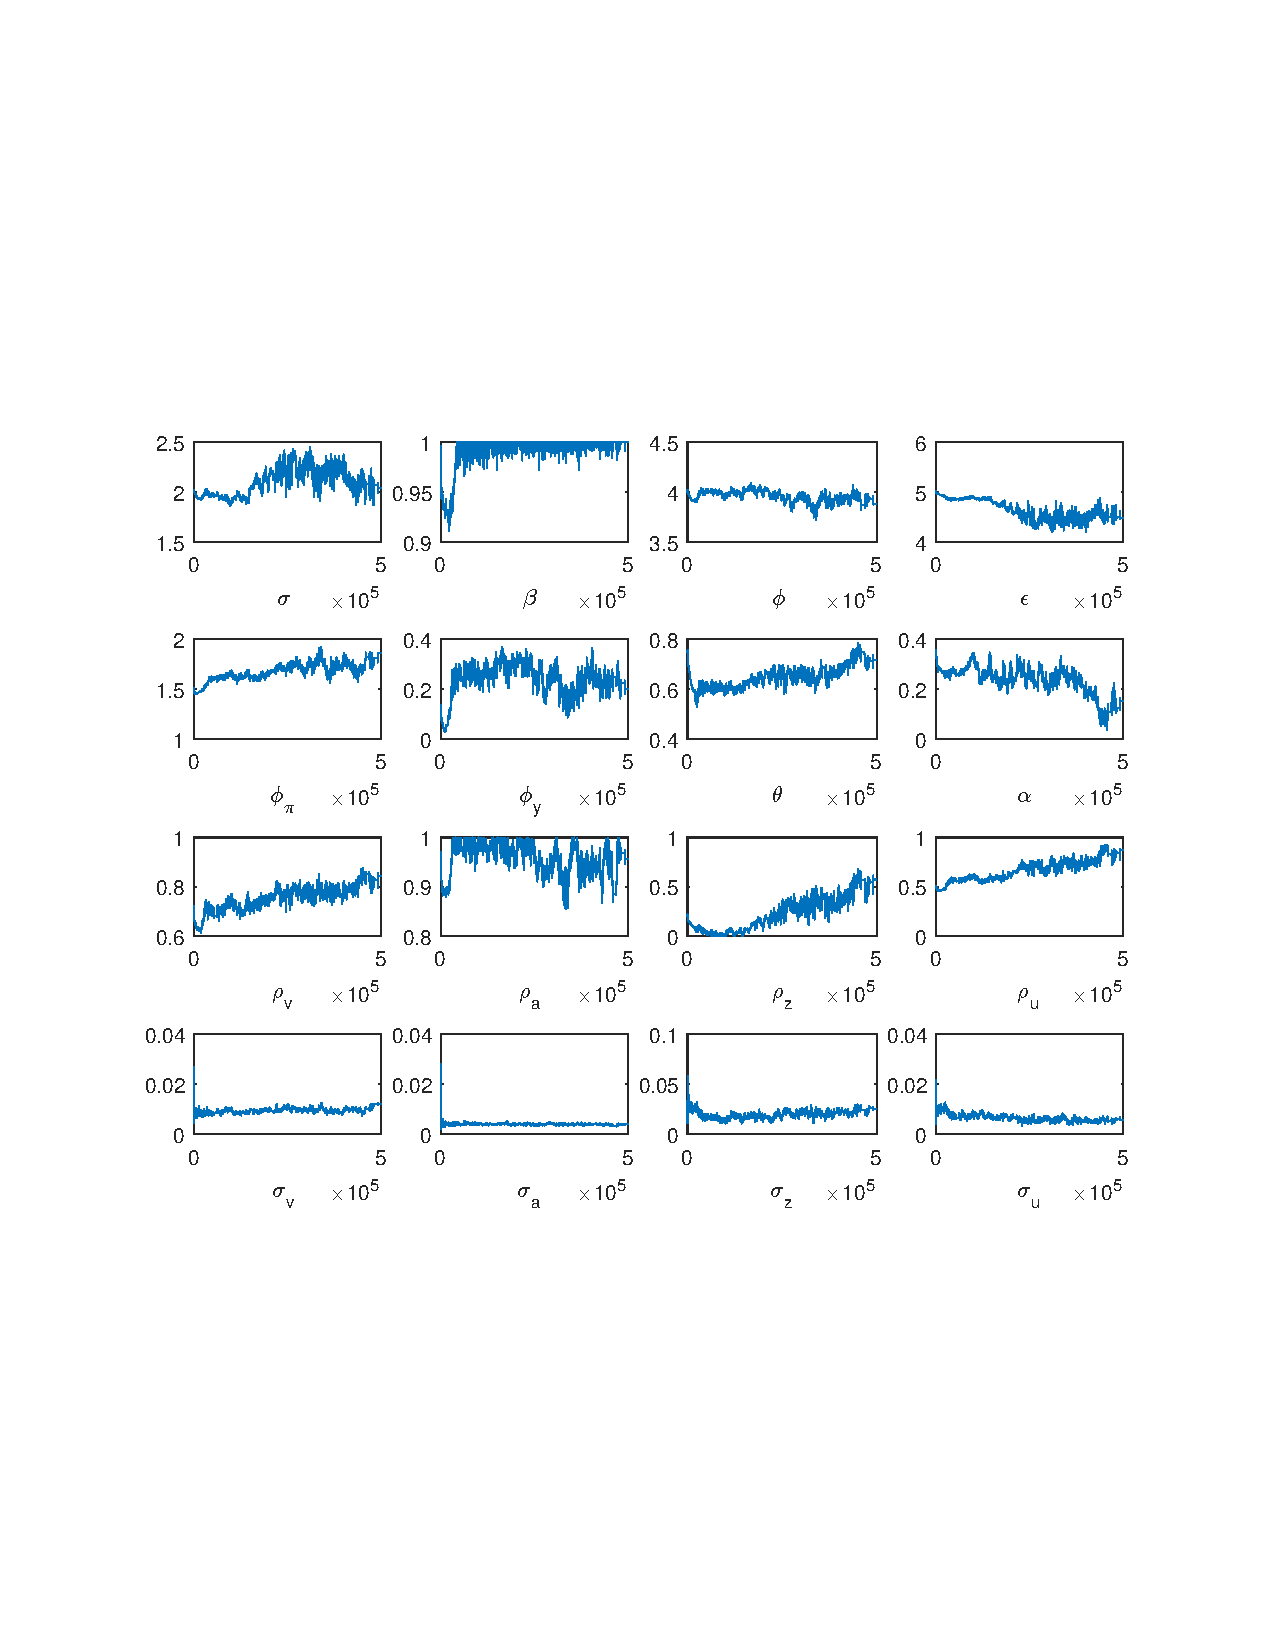
\includegraphics[width=\linewidth]{raw_MCMC}
	\caption{Raw MCMC of $\Theta$}
	\label{fig:raw}
\end{figure}

It usually a good idea to discard the first part of the Markov Chain since it takes some time before the algorithm reaches the stationary distribution. The raw MCMC for $\Theta$ with a burn-in sample of 20\% is plotted in Fig. \ref{fig:burn}.

\begin{figure}[H]
	\centering
	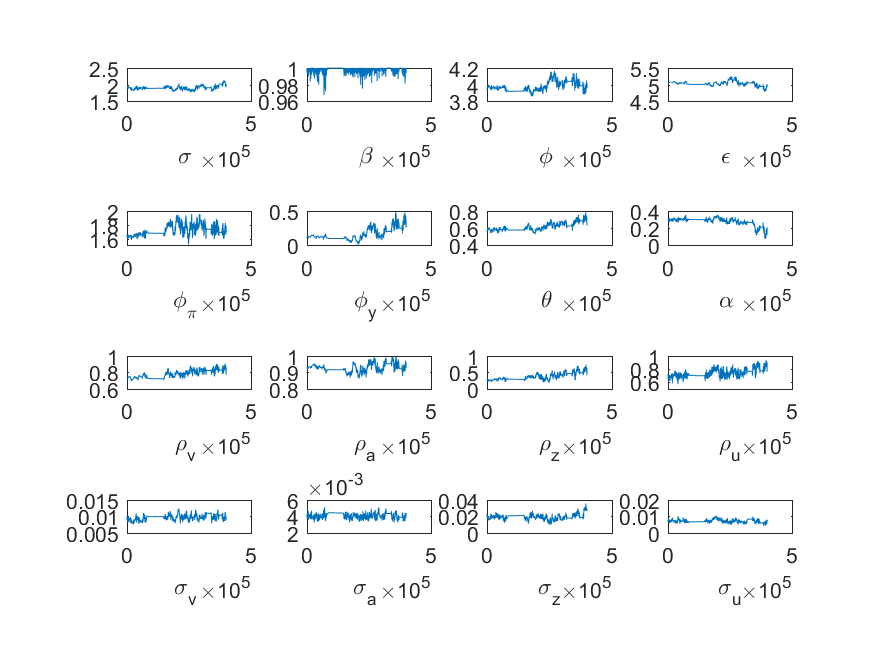
\includegraphics[width=\linewidth]{burn_MCMC}
	\caption{MCMC of $\Theta$ with discarded burn-in sample}
	\label{fig:burn}
\end{figure}

Finally, to check for convergence, it is easier to look at the cumulative mean and see if it stabilizes. The cumulative mean of the MCMC for $\Theta$ is plotted in Fig. \ref{fig:conv}. It is straightforward to see that the cumulative mean stabilizes for every single component of $\Theta$, hence we have convergence.
\begin{figure}[H]
	\centering
	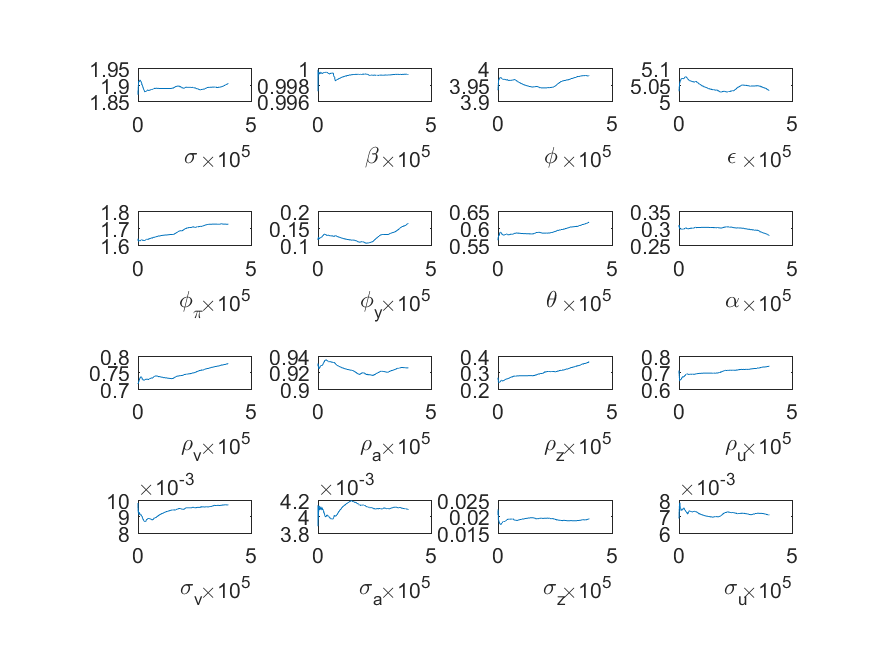
\includegraphics[width=\linewidth]{conv_MCMC}
	\caption{Cumulative mean of $\Theta$}
	\label{fig:conv}
\end{figure}


\section*{Part (3)}
The posterior distribution of $\Theta$ is plotted in Fig. \ref{fig:dist}.

\begin{figure}[H]
	\centering
	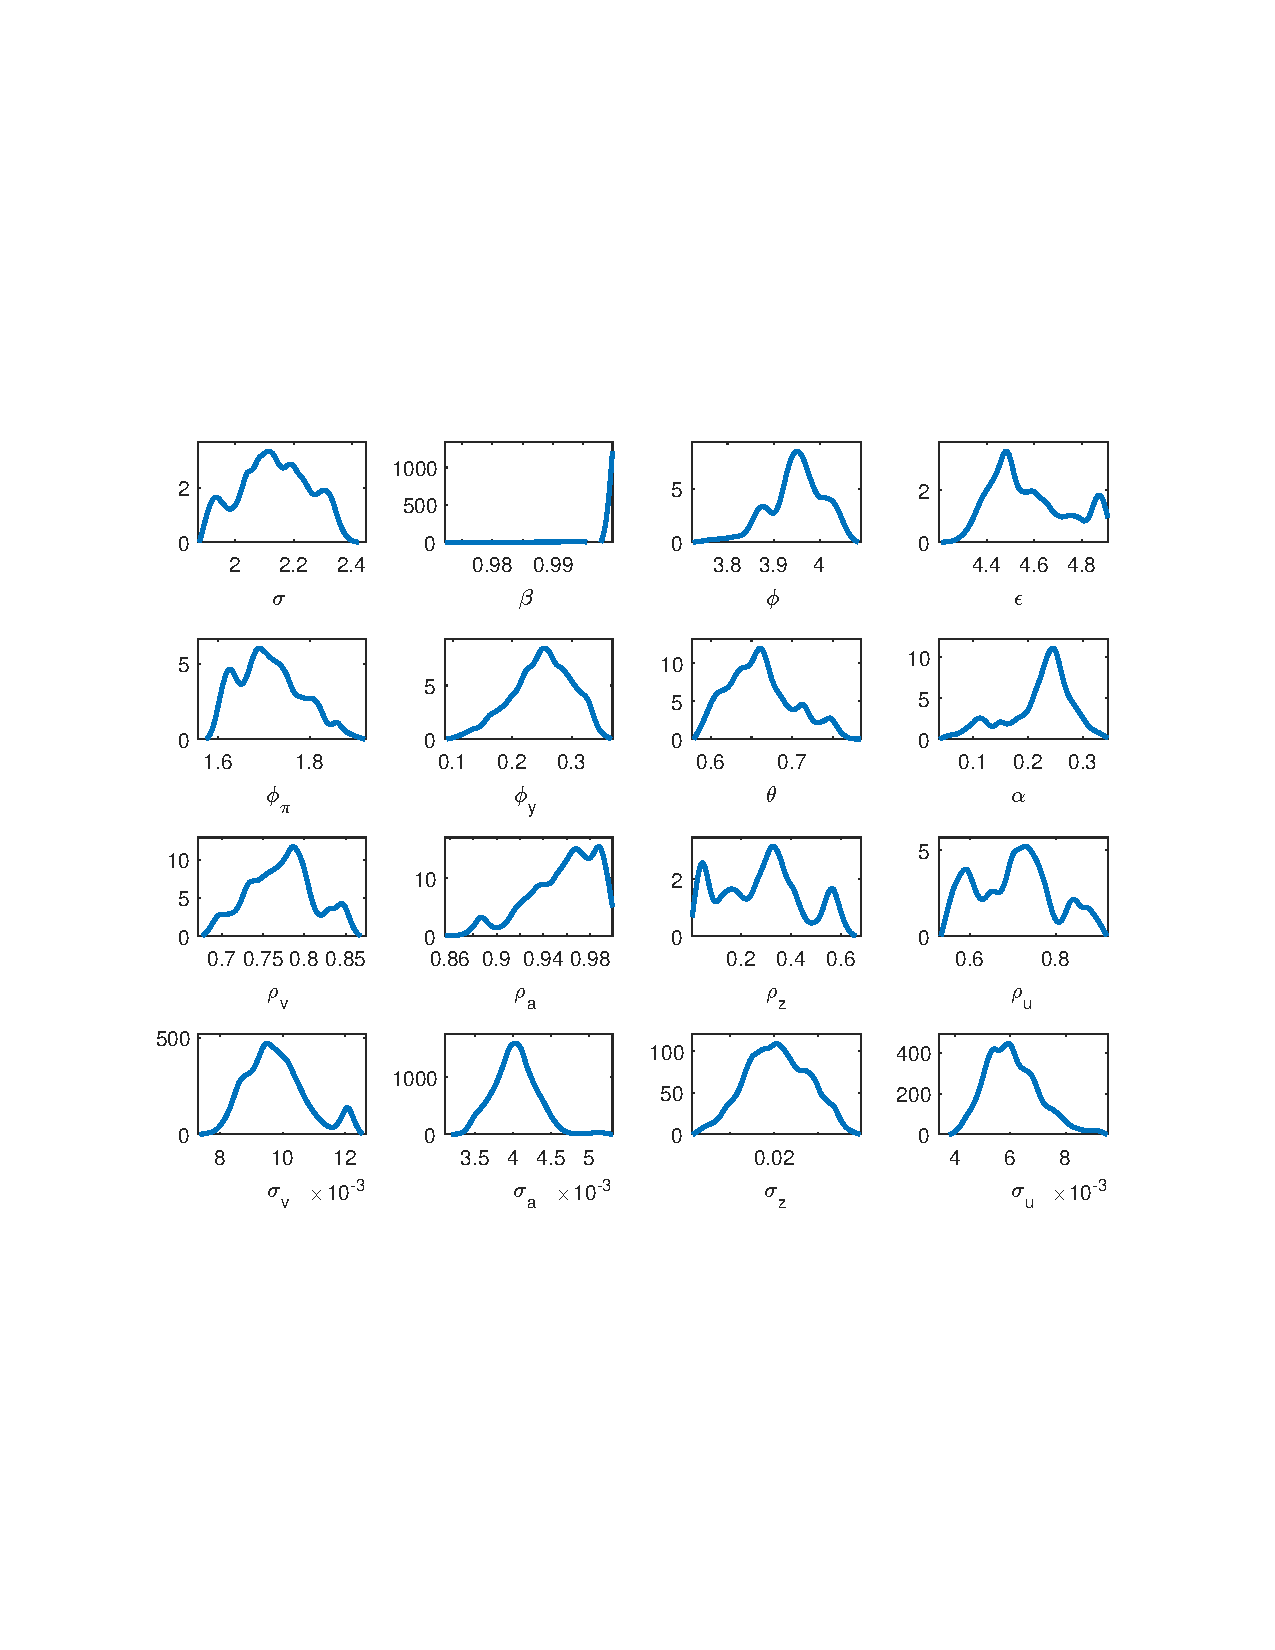
\includegraphics[width=\linewidth]{dist_MCMC}
	\caption{Posterior distribution of $\Theta$}
	\label{fig:dist}
\end{figure}


\section*{Part (4)}

The impulse responses are plotted in Fig.\ref{fig:impulse_monetary}, Fig.\ref{fig:impulse_prod}, Fig.\ref{fig:impulse_demand} and Fig.\ref{fig:impulse_cost}.


\begin{figure}[H]
	\centering
	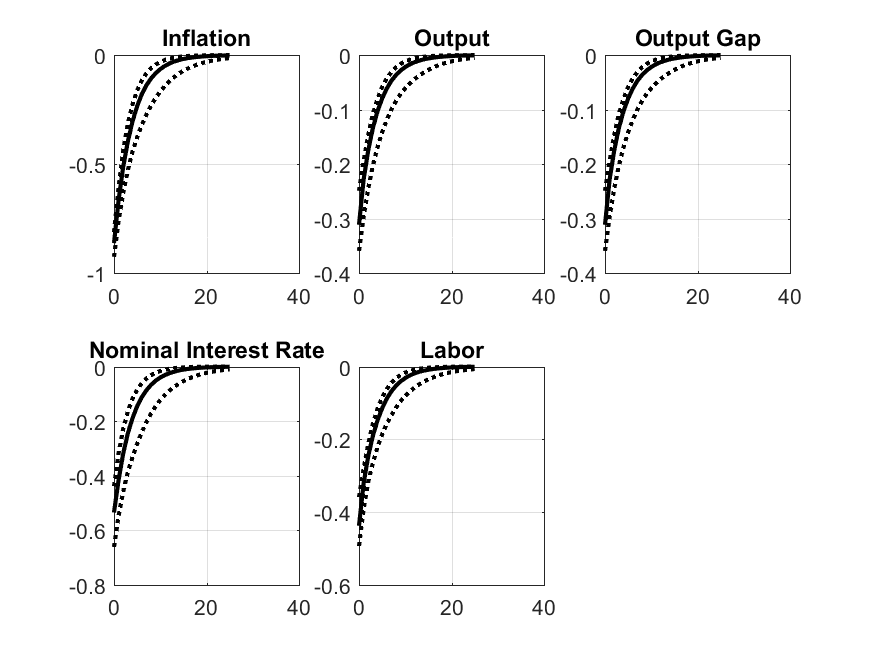
\includegraphics[width=\linewidth, height = 0.4\textheight]{impulse_monetary}
	\caption{Impulse response to monetary shocks}
	\label{fig:impulse_monetary}
\end{figure}
\begin{figure}[H]
	\centering
	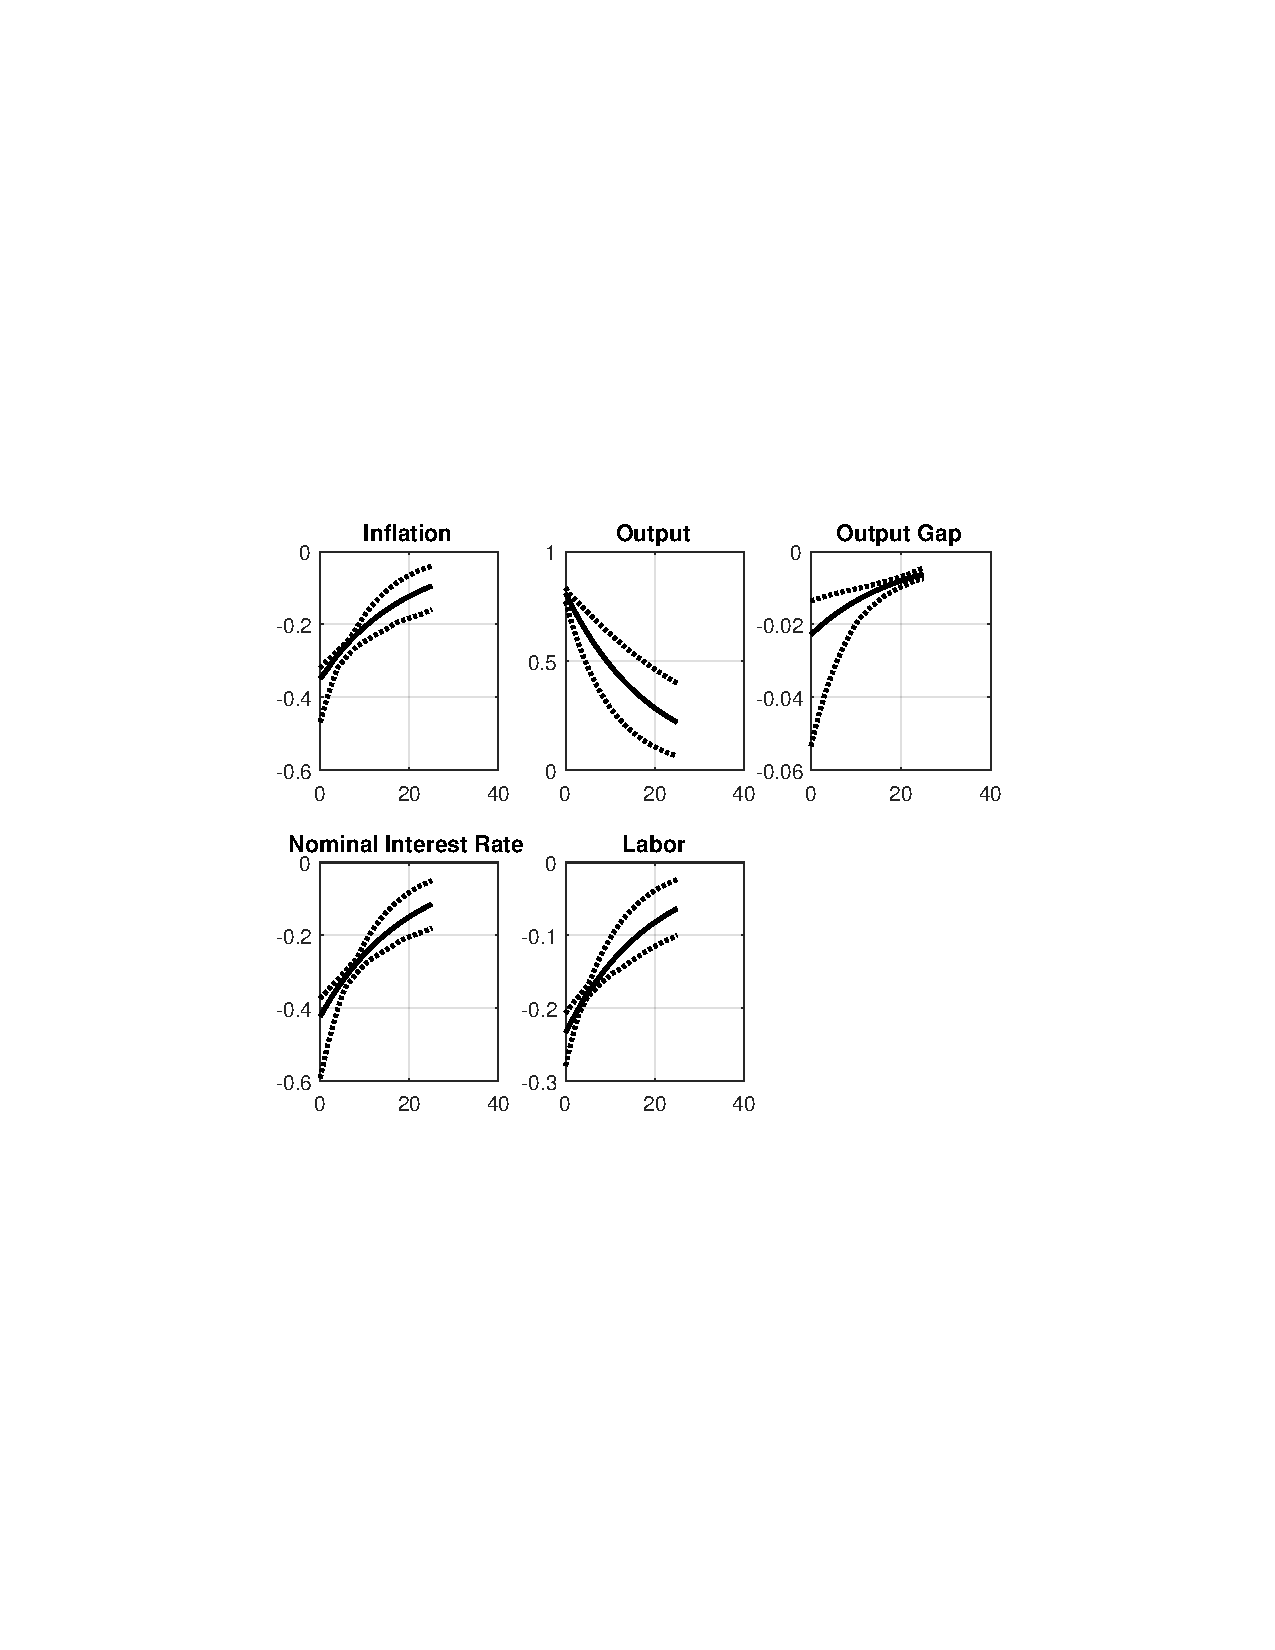
\includegraphics[width=\linewidth, height = 0.4\textheight]{impulse_prod}
	\caption{Impulse response to productivity shocks}
	\label{fig:impulse_prod}
\end{figure}
\begin{figure}[H]
	\centering
	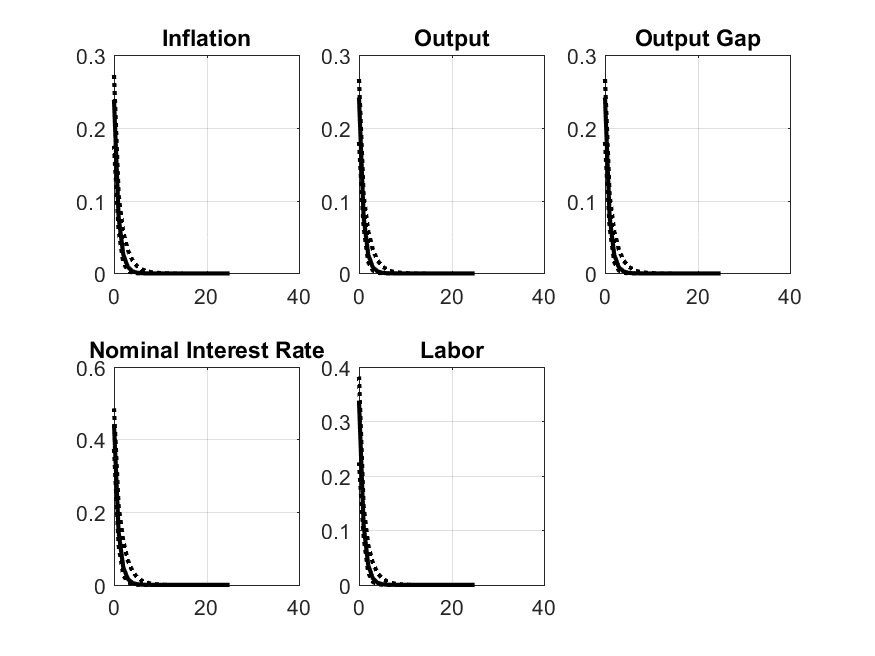
\includegraphics[width=\linewidth, height = 0.4\textheight]{impulse_demand}
	\caption{Impulse response to demand shocks}
	\label{fig:impulse_demand}
\end{figure}
\begin{figure}[H]
	\centering
	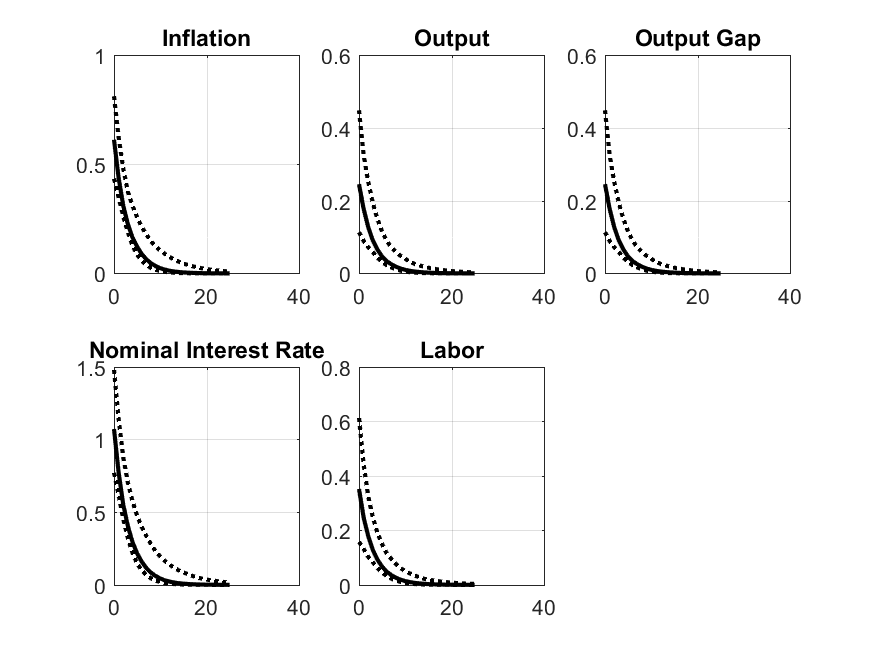
\includegraphics[width=\linewidth, height = 0.4\textheight]{impulse_cost}
	\caption{Impulse response to cost-push shocks}
	\label{fig:impulse_cost}
\end{figure}

\section*{Part (5)}

The distribution of the variance decomposition of each observable variable are plotted in Fig.\ref{fig:var_monetary}, Fig.\ref{fig:var_prod}, Fig.\ref{fig:var_demand} and Fig.\ref{fig:var_cost}.

\begin{figure}[H]
	\centering
	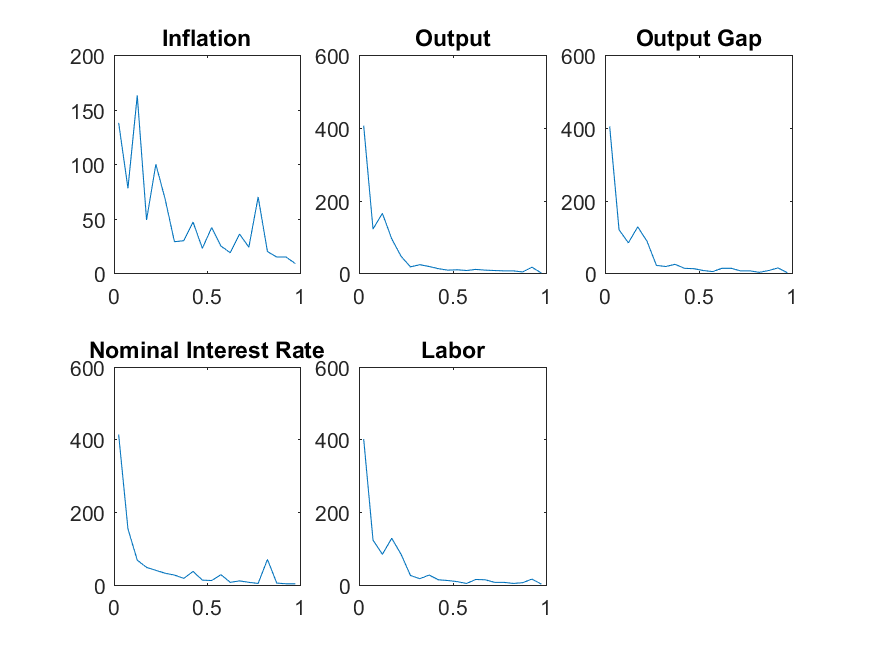
\includegraphics[width=\linewidth, height = 0.4\textheight]{var_monetary}
	\caption{Variance decomposition - Monetary shocks}
	\label{fig:var_monetary}
\end{figure}
\begin{figure}[H]
	\centering
	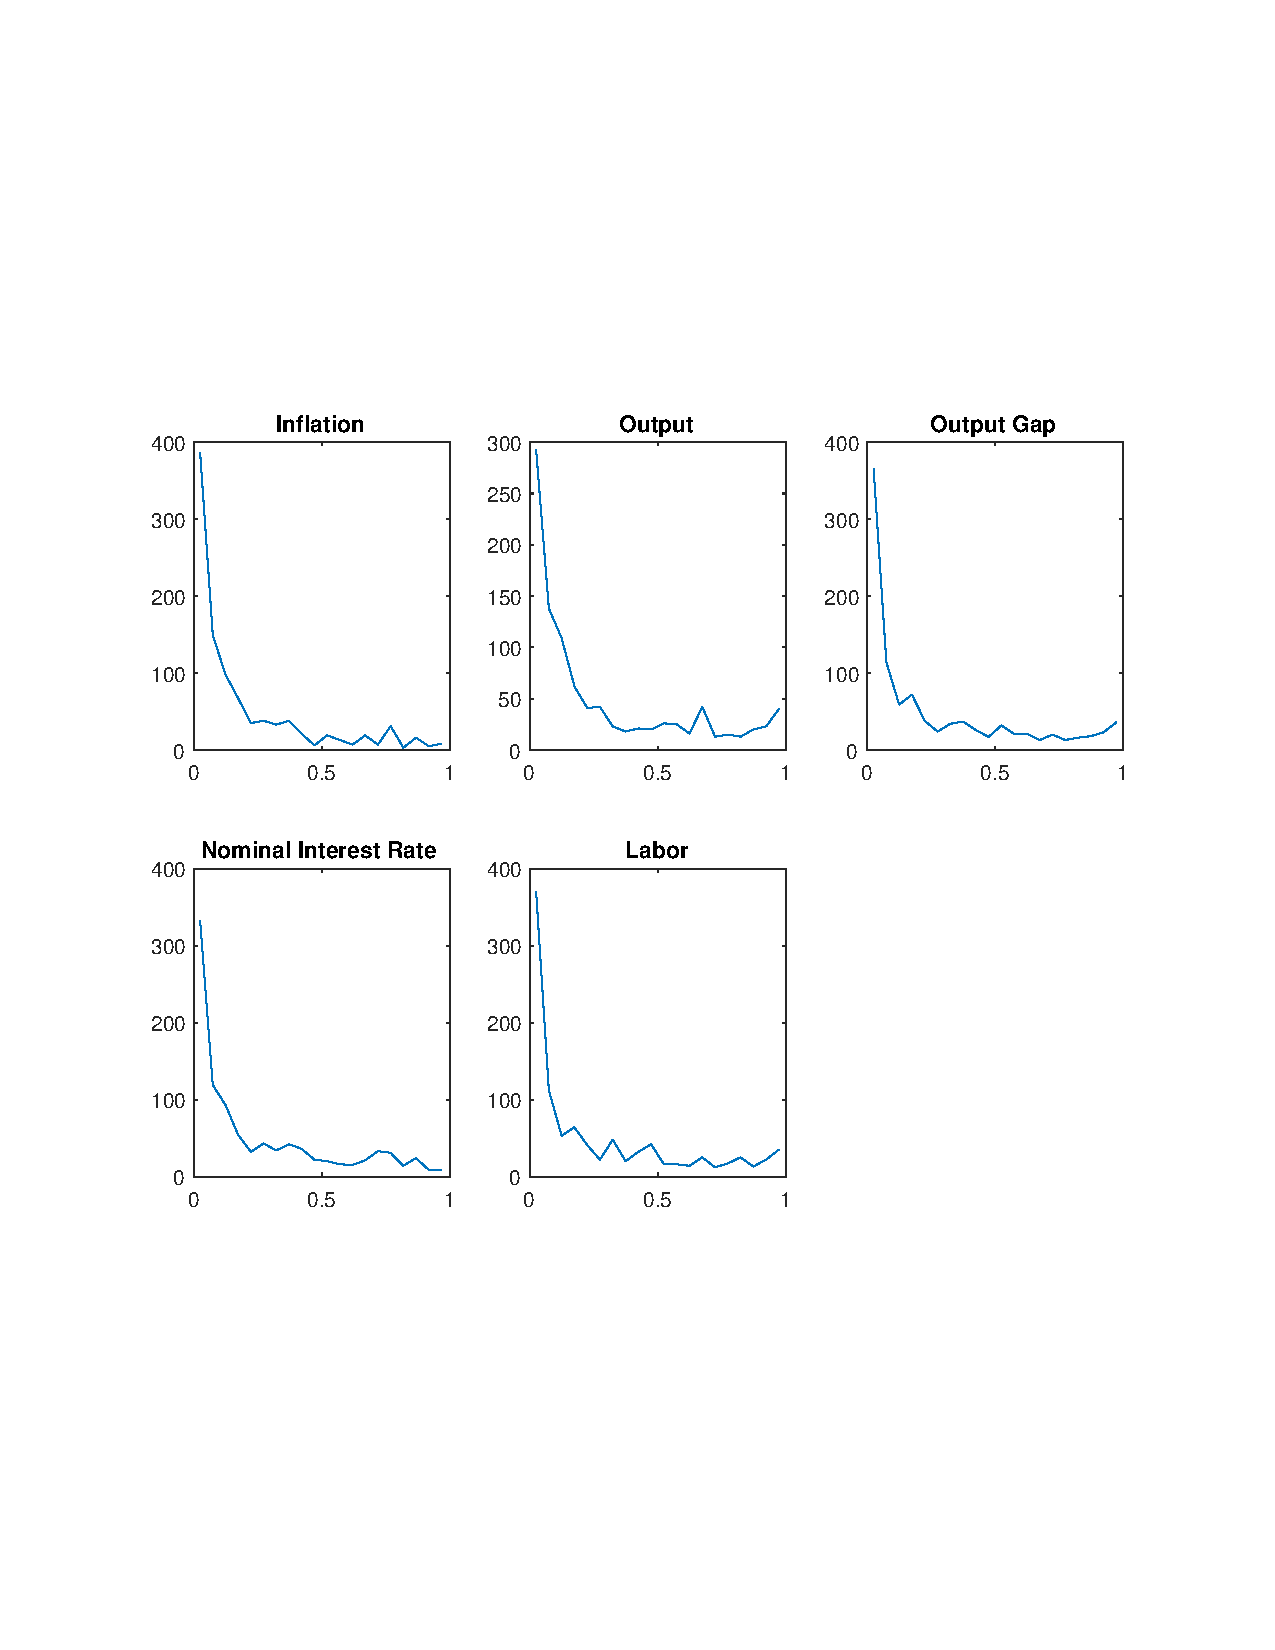
\includegraphics[width=\linewidth, height = 0.4\textheight]{var_prod}
	\caption{Variance decomposition - Productivity shocks}
	\label{fig:var_prod}
\end{figure}
\begin{figure}[H]
	\centering
	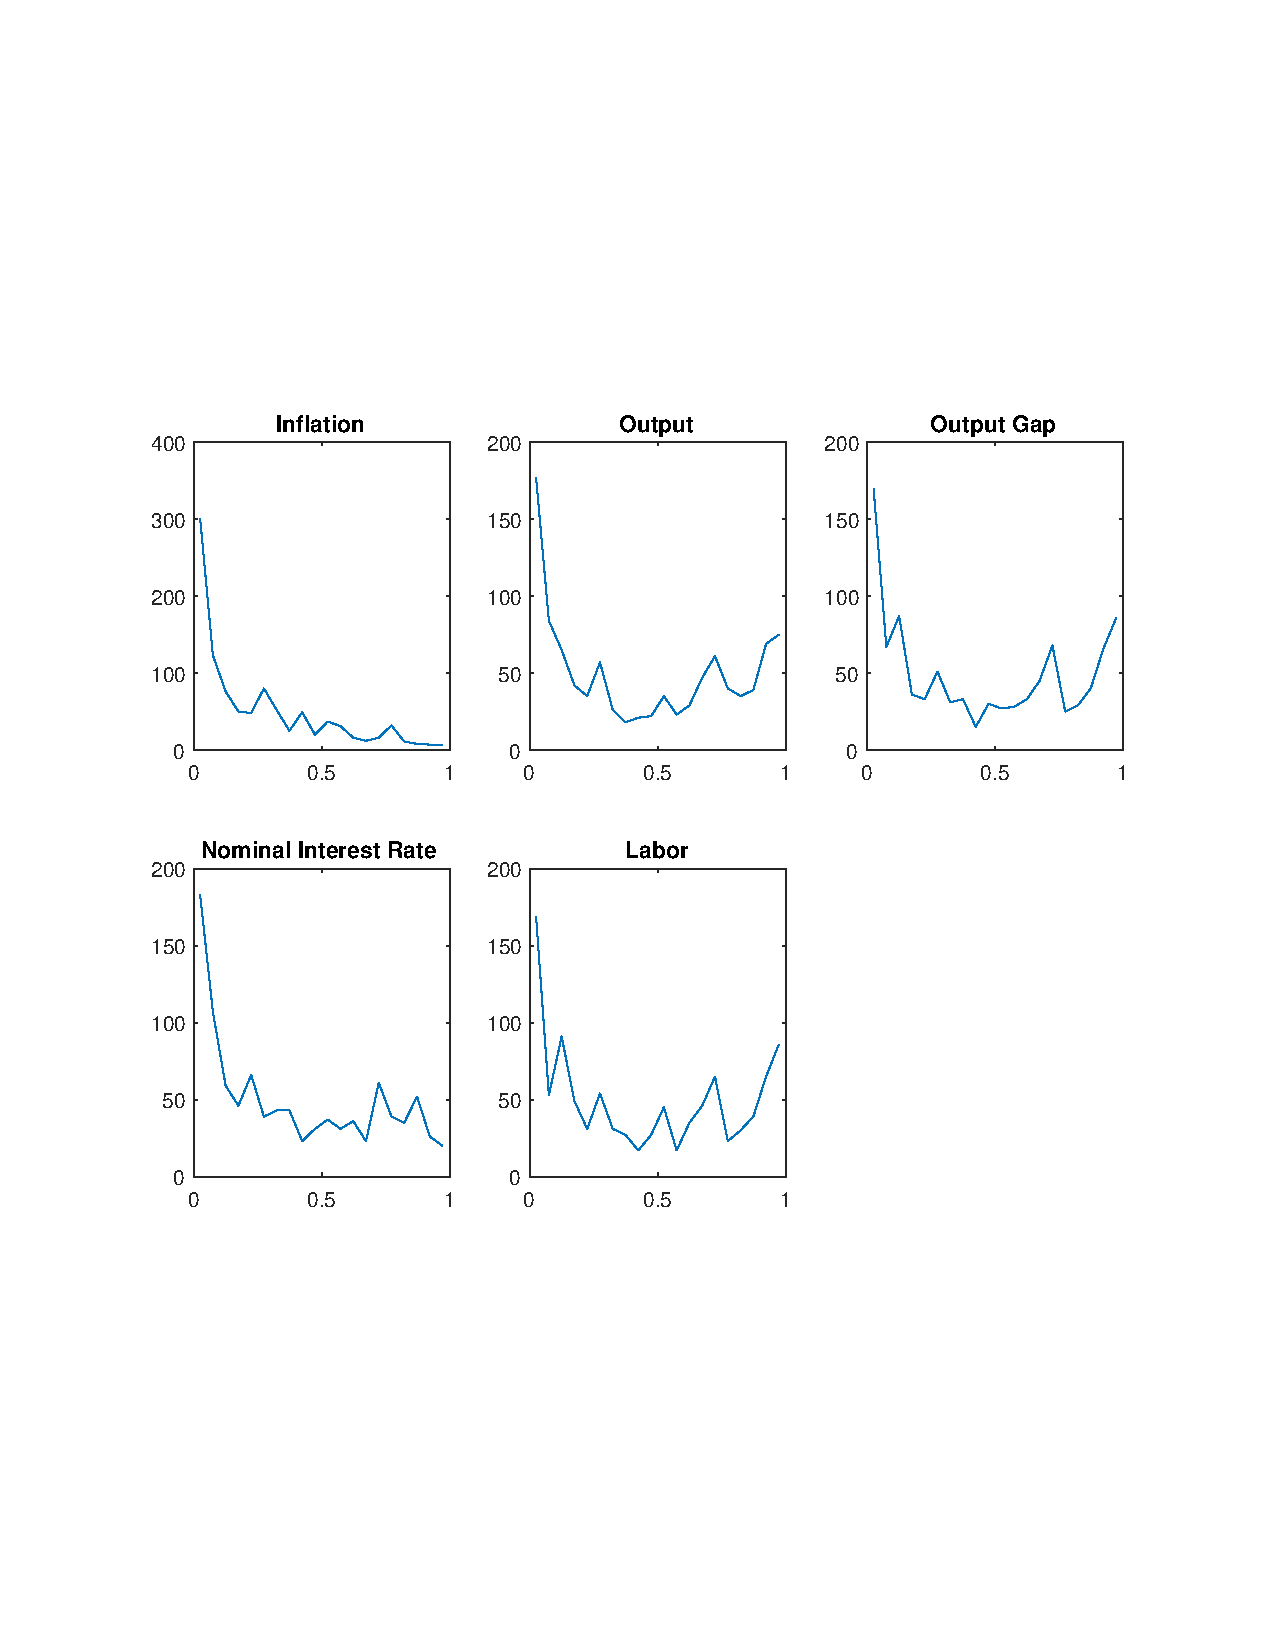
\includegraphics[width=\linewidth, height = 0.4\textheight]{var_demand}
	\caption{Variance decomposition - Demand shocks}
	\label{fig:var_demand}
\end{figure}
\begin{figure}[H]
	\centering
	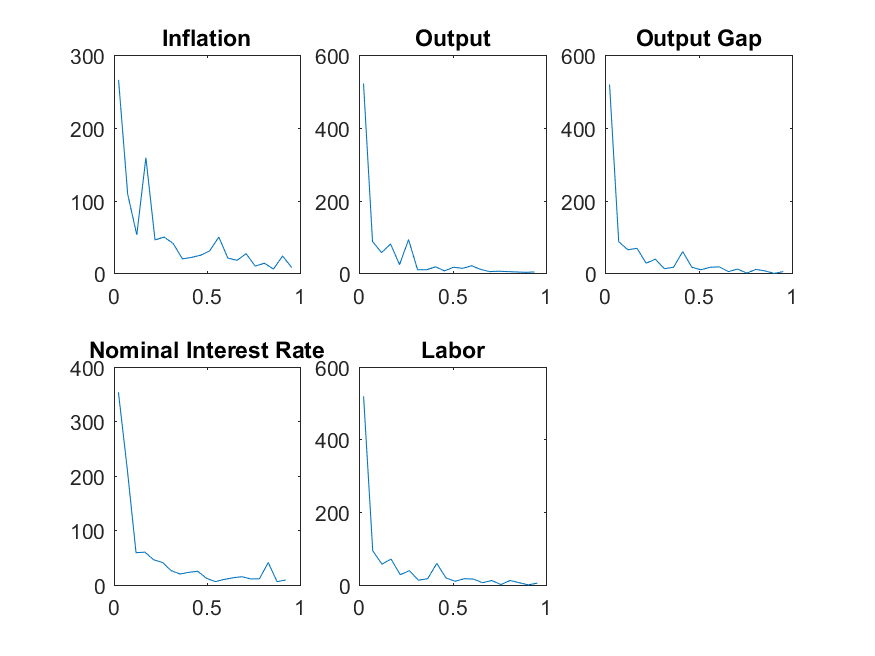
\includegraphics[width=\linewidth, height = 0.4\textheight]{var_cost}
	\caption{Variance decomposition - Cost-push shocks}
	\label{fig:var_cost}
\end{figure}


\section*{Part (6)}
Using a sample of 1000 points from our Markov Chain, we compute the posterior probability that labor inputs fall for 8 consecutive quarters after a positive productivity shock
\[
P(\text{labor inputs in 8 consecutive quarters}<0 \mid Z) = 1
\]
i.e. it always falls.

\section*{Code}
\subsubsection*{Main (main.m)}
\lstinputlisting[language=Matlab]{main.m}
\subsubsection*{New Keynesian Model (nkbc\_model.m)}
\lstinputlisting[language=Matlab]{NKBC_model.m}

\subsubsection*{Loglikelihood - Data (LLDSGE.m)}
\lstinputlisting[language=Matlab]{LLDSGE.m}

\subsubsection*{Loglikelihood - Prior (log\_prior\_DSGEmodel.m)}
\lstinputlisting[language=Matlab]{log_prior_DSGE.m}

\subsubsection*{Plot - Raw Data (plotraw.m)}
\lstinputlisting[language=Matlab]{plotraw.m}

\subsubsection*{Plot - Cumulative Mean (convcheck.m)}
\lstinputlisting[language=Matlab]{convcheck.m}

\subsubsection*{Plot - Distribution (plotpost.m)}
\lstinputlisting[language=Matlab]{plotpost.m}

\subsubsection*{Kalman Filter (kfilter.m)}
\lstinputlisting[language=Matlab]{kfilter.m}

\end{document}
